\documentclass{article}

\usepackage[utf8]{inputenc}
\usepackage[danish]{babel}
\usepackage{float}
\usepackage{fancyhdr}
\usepackage{amsmath}
\usepackage{color}
\usepackage{listings}
\usepackage{graphicx}
\usepackage{pdfpages}
\usepackage{booktabs}
\usepackage{listingsutf8}
%\usepackage{enumitem}
\usepackage[a4paper, top = 1in, bottom = 1in, left=1in,right=1in]{geometry}

\title{Tællende Aktivitet 2}
\author{Peter Heilbo Ratgen \\ perat17}
\date{\today}

\begin{document}
\maketitle

\section{Opgave 1}
\subsection{Deskriptiv analyse}
En deskriptiv analyse af udgifterne til behandling af patienter 
\textsc{Treatcost} 

\begin{figure}[h]
  \centering
  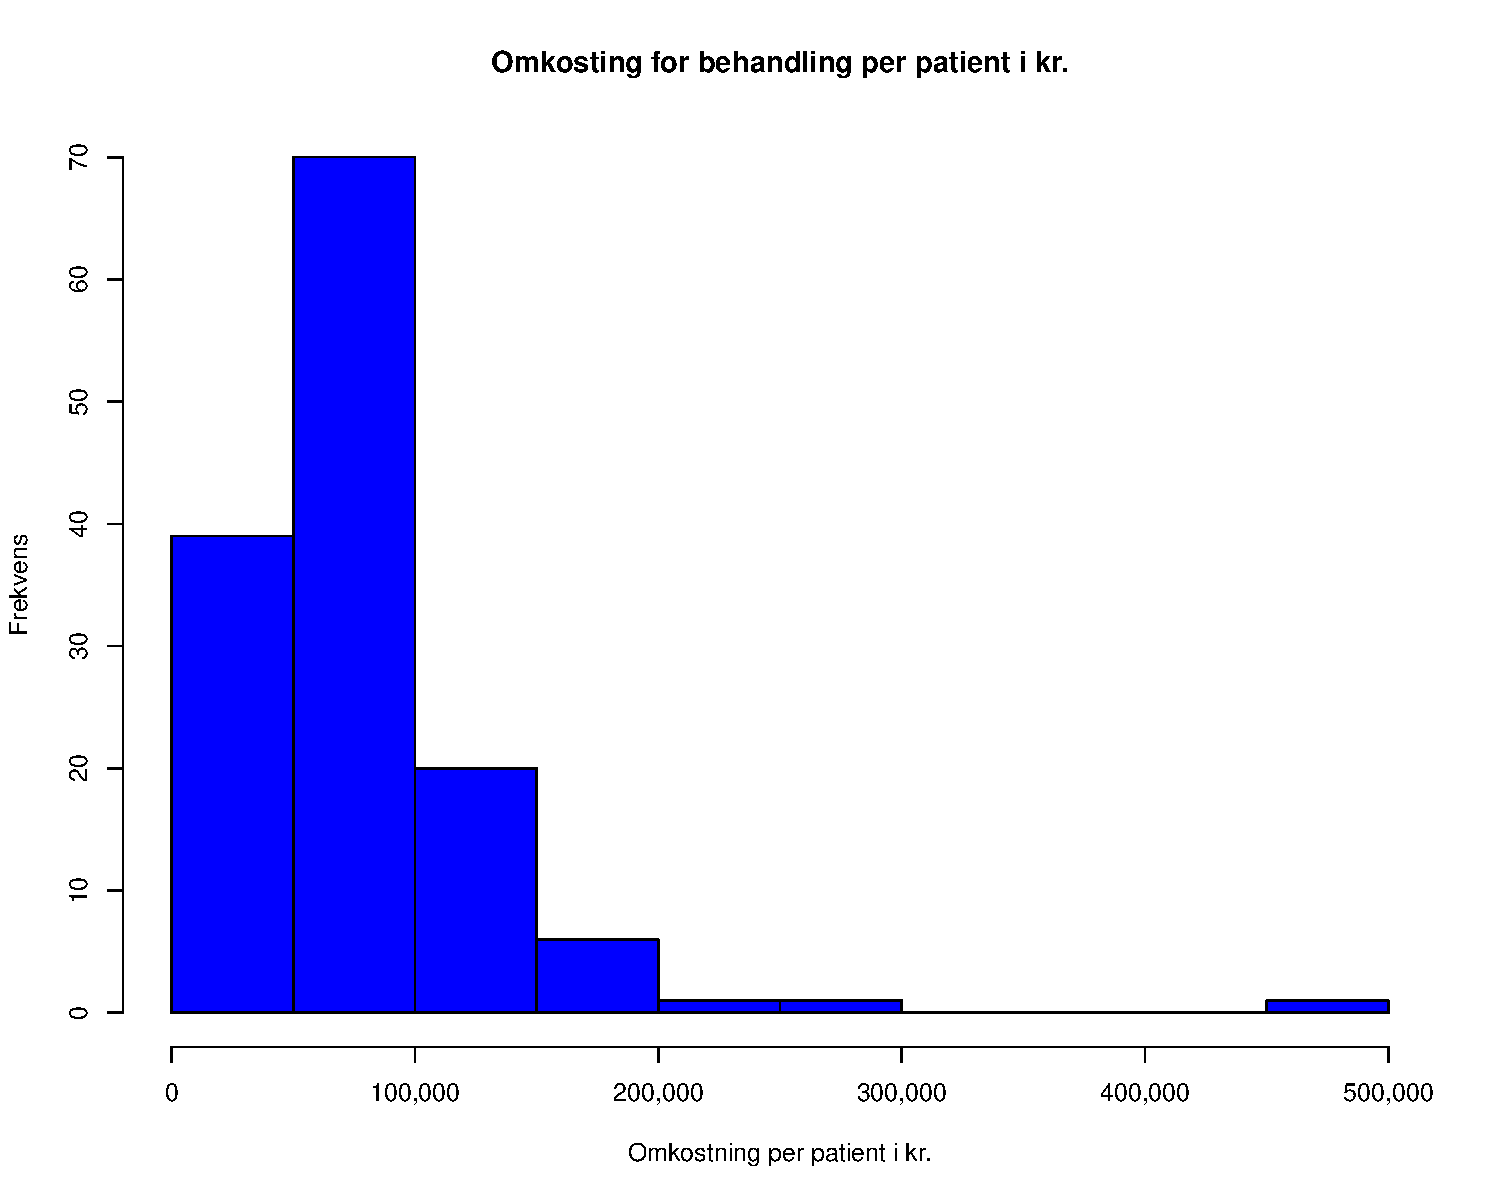
\includegraphics[width=0.6\textwidth]{./plots/treatcost.pdf}
  \caption{Histogram af omkostningen for at behandle patienter}
\end{figure}

\begin{table}[H]
  \begin{tabular}{l|l}
    Gennemsnit        &  78754\\\hline
    Median            &  65992 \\\hline
    Typeinterval (modus)     & 50000 - 10000  \\\hline
    Standardafvigelse &  55608.07\\\hline
    Standard error    &  4733.673 \\\hline
    Minimum           & 17989  \\\hline
    Maximum           &  492833 \\\hline
    $Q_1$             &  46202\\\hline
    $Q_3$             & 91328 
  \end{tabular}
\end{table}

Ved at se på histogram og median samt gennemsnit ses at formen er højreskæv.
Formen er på histogrammet er ikke symmetrisk. Hvis man betrager nedenstående
boxplot ses det at der er en ekstrem observation. Der falder langt uden for
andre observationer. Selvom dette er en outlier er dette datapunkt stadig vigtig
at have med.

\begin{figure}[H]
  \centering
  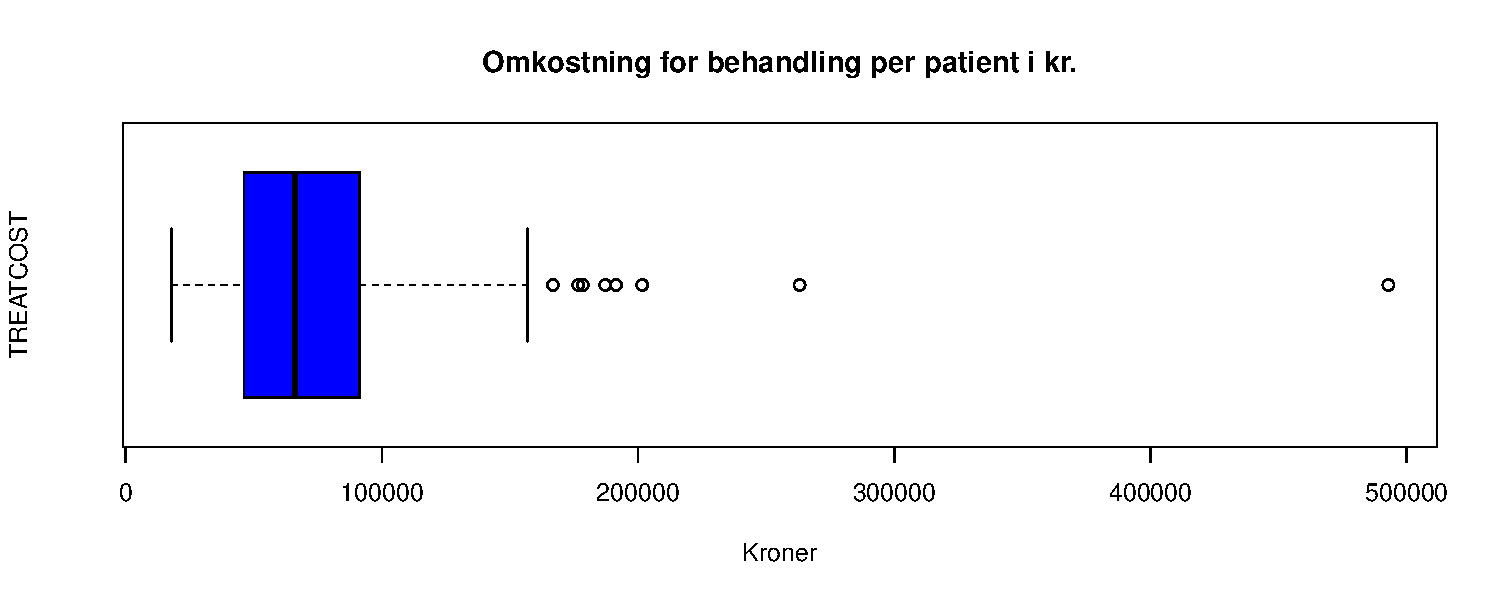
\includegraphics[width=0.8\textwidth]{./plots/costboxplot.pdf}
  \caption{Boxplot af omkostning for at behandle patienter}
\end{figure}

\subsection{Konfidensinterval for middelværdien}
Vi opstiller et konfidensinterval på 95\%. Dette betyder at 95\% af data vil
falde inden for dette interval.
Vi udregner konfidensintervallet ved, at finde gennemsnittet og
standardafvigelsen og vi anvender qnorm til at finde $ Z $ -scoren for den givne
andel af observationsættet. Ud fra denne værdi kan konfidensintervallet ved at
fratrække fejlmargenen fra gennemsnitsværdien.

Da ender vi med et konfidensinterval $ [69476.61:88032.26] $, her ligger 95\%
fra værdierne.

\subsection{Sandsynlighed for samlede udgifter}
Sandsynligheden for at en behandling kommer til at koste over 95.000 kr. er
givet ved \[
\frac{\text{antal behandlinger over 95000}}{\text{antal behandlinger i alt}} =
\frac{34}{138} = 0.2463768
.\] 

\subsection{Sandsynlighed for samlede udgifter mellem 40000 og 65000}
Sandsynlighed for at en behandling kommer til at koste mellem 40,000 og 65,000
er givet ved: 
\[
1 - \frac{\text{antal behandlinger under 40000} + \text{antal behandlinger over
65000}}{\text{antal behandlinger}}
.\] 

Da får vi:
\[
1 - \frac{21 + 70 }{138} = 0.3405797
.\] 
\section{Opgave 2}

Vi stater med at lave et scatterplot for at få et overblik over data:
\begin{figure}[H]
  \centering
  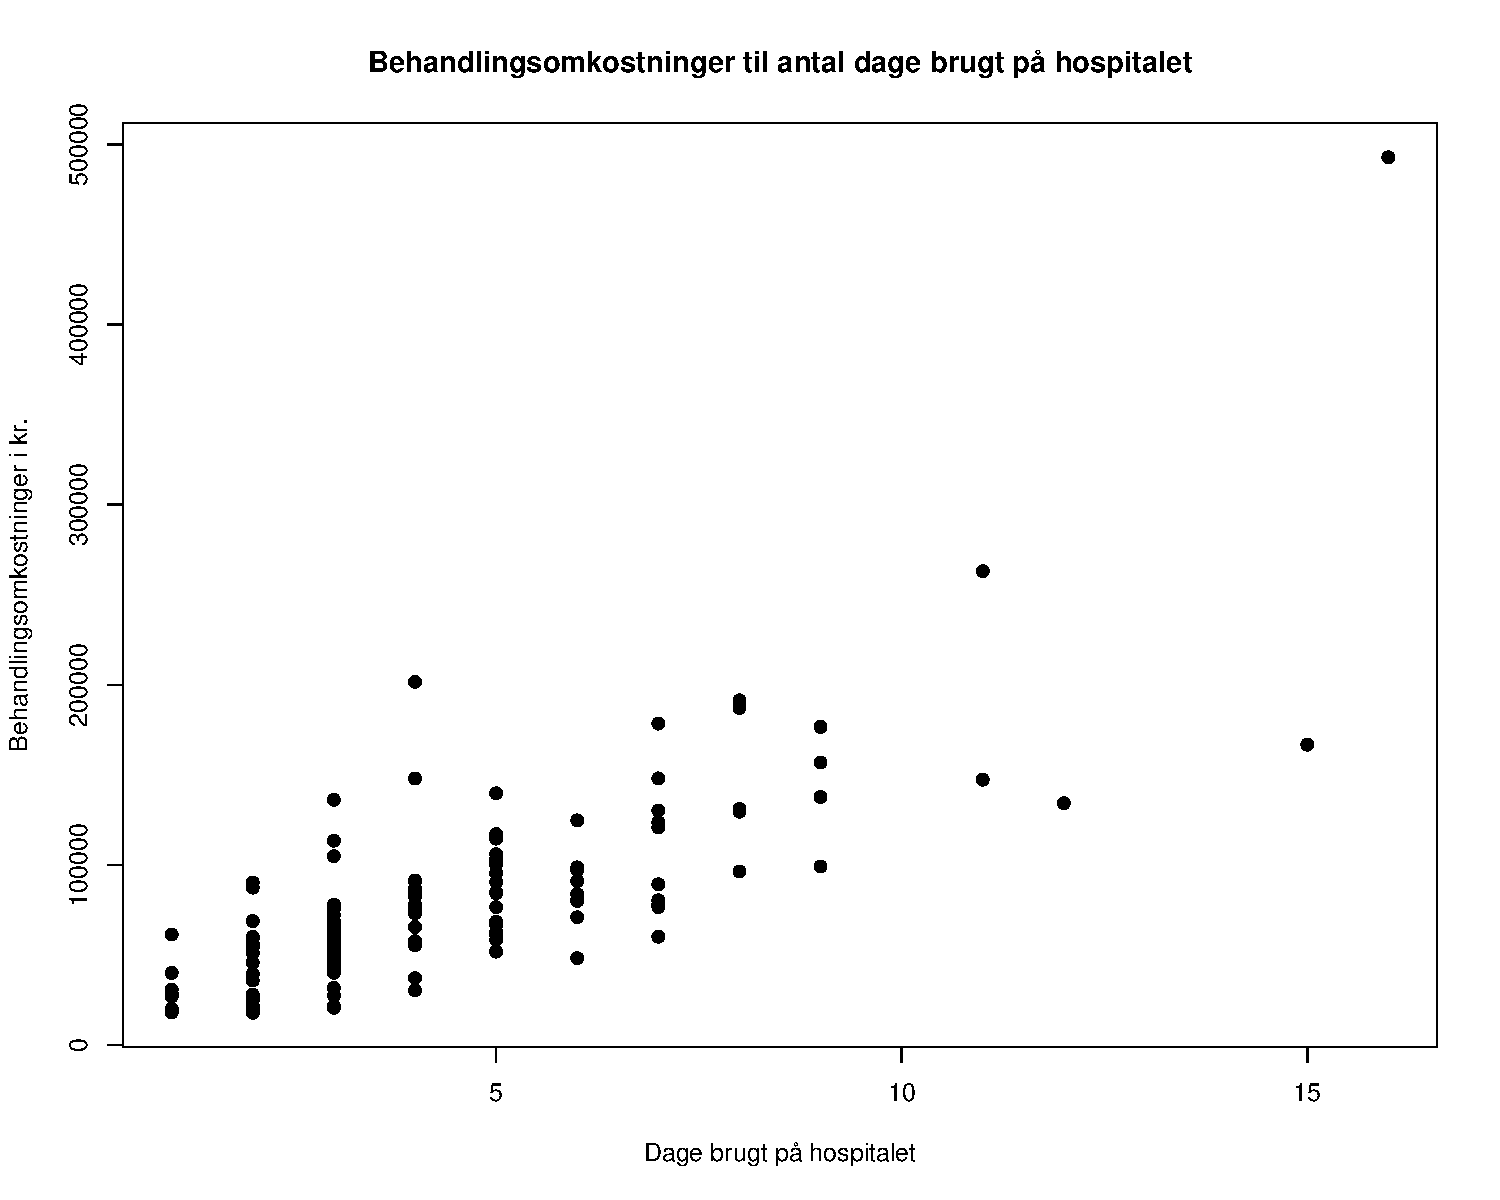
\includegraphics[width=0.6\textwidth]{./plots/caredaysScatterPlot.pdf}
  \caption{Scatterplot over dage på hospitalet og dennes sammenhæng med
  behandlindsomkostninger}
\end{figure}

Vi laver en regression på formen 
\[
TREATCOST_i = \beta_0 + \beta_1CAREDAYS_i + \epsilon_i \quad i = 1,\dots,138
.\] 
Dette giver denne regressionslinjre

\begin{figure}[H]
  \centering
  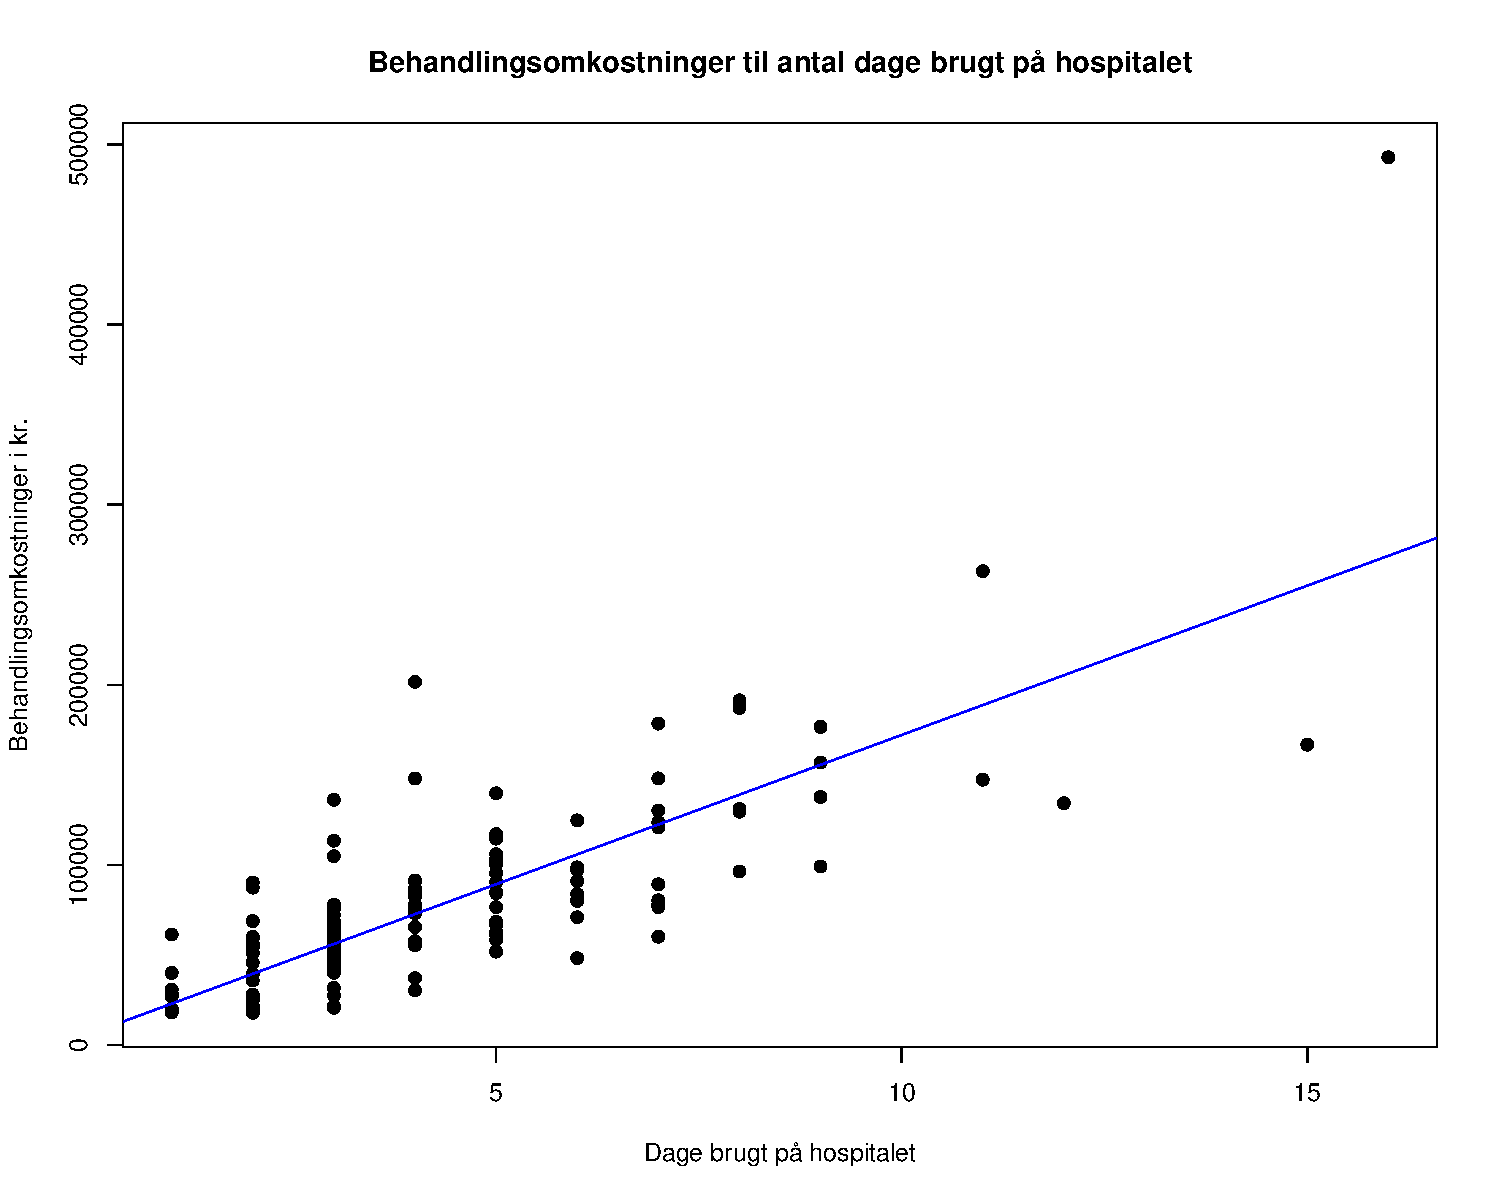
\includegraphics[width=0.6\textwidth]{./plots/caredaysScatterPlotAbline.pdf}
  \caption{Scatterplot over dage på hospitalet og dennes sammenhæng med
  behandlindsomkostninger}
\end{figure}

Vi kigger på residulerne for regressionslinjen: 

\begin{figure}[H]
  \centering
  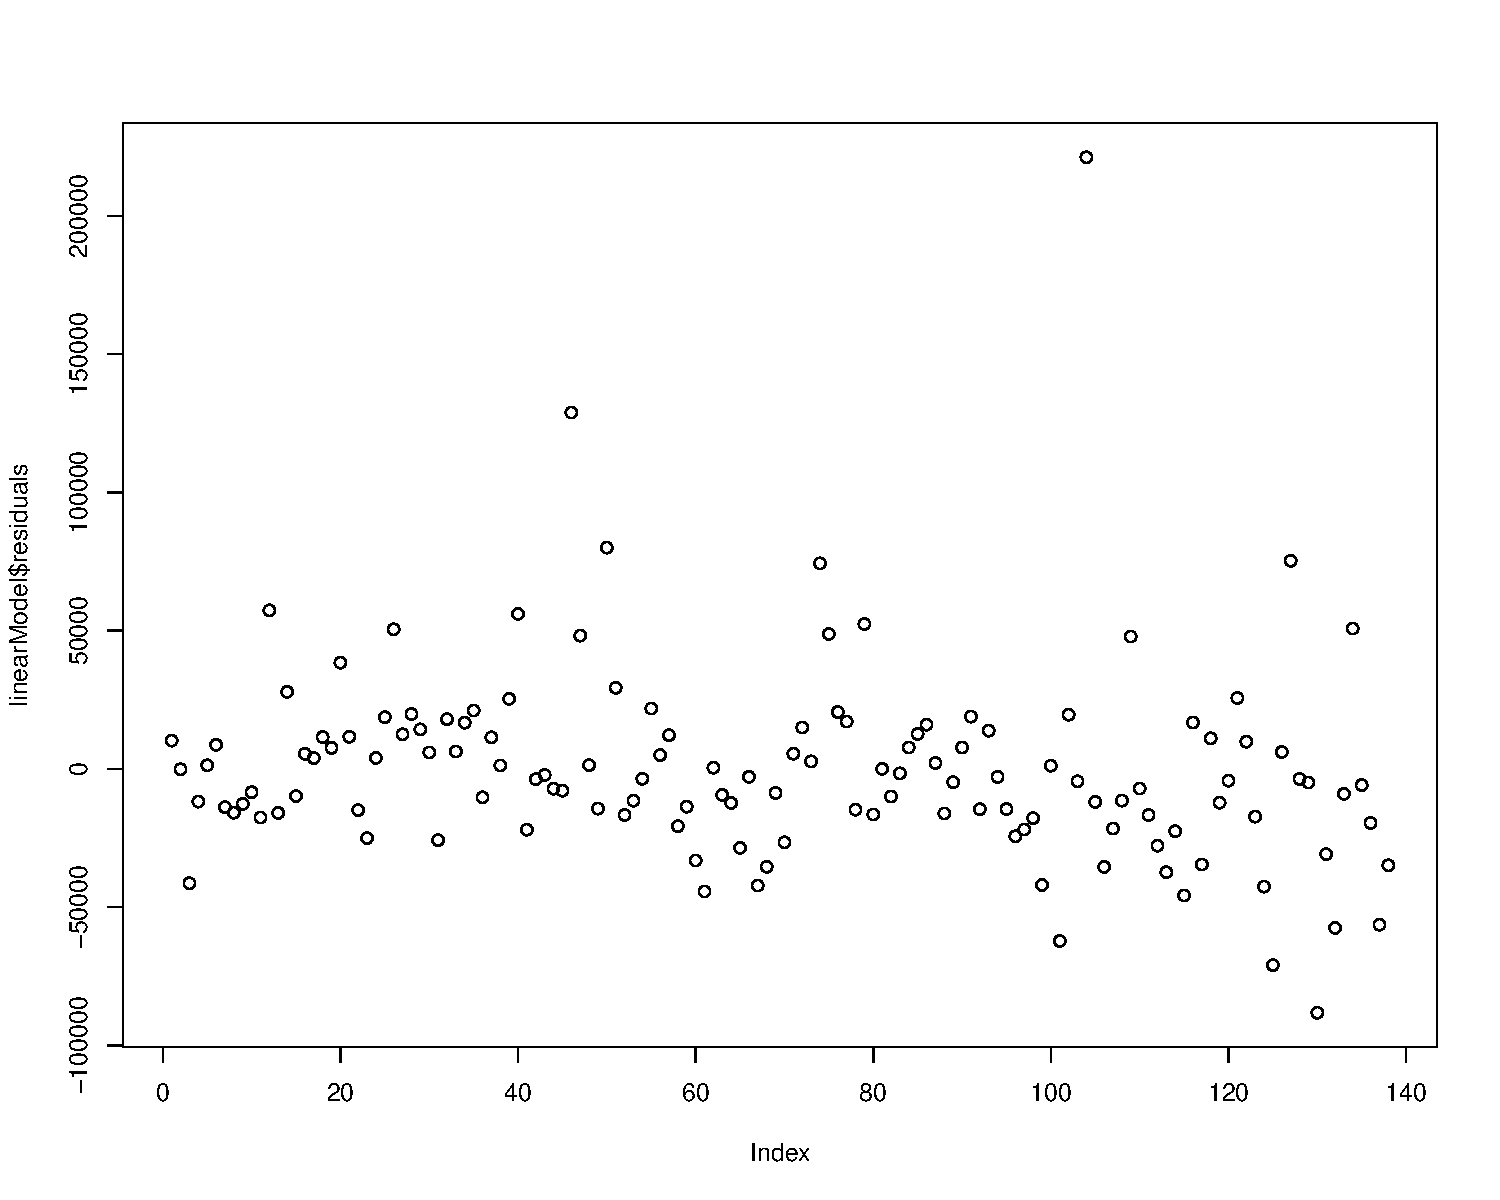
\includegraphics[width=0.6\textwidth]{./plots/caredaysResiduals.pdf}
  \caption{caption}
\end{figure}

Hvis vi kigger på residualerne de betegnes som tilfældige, der er dog en ekstrem
observation som også set tidligere.

\begin{figure}[H]
  \centering
  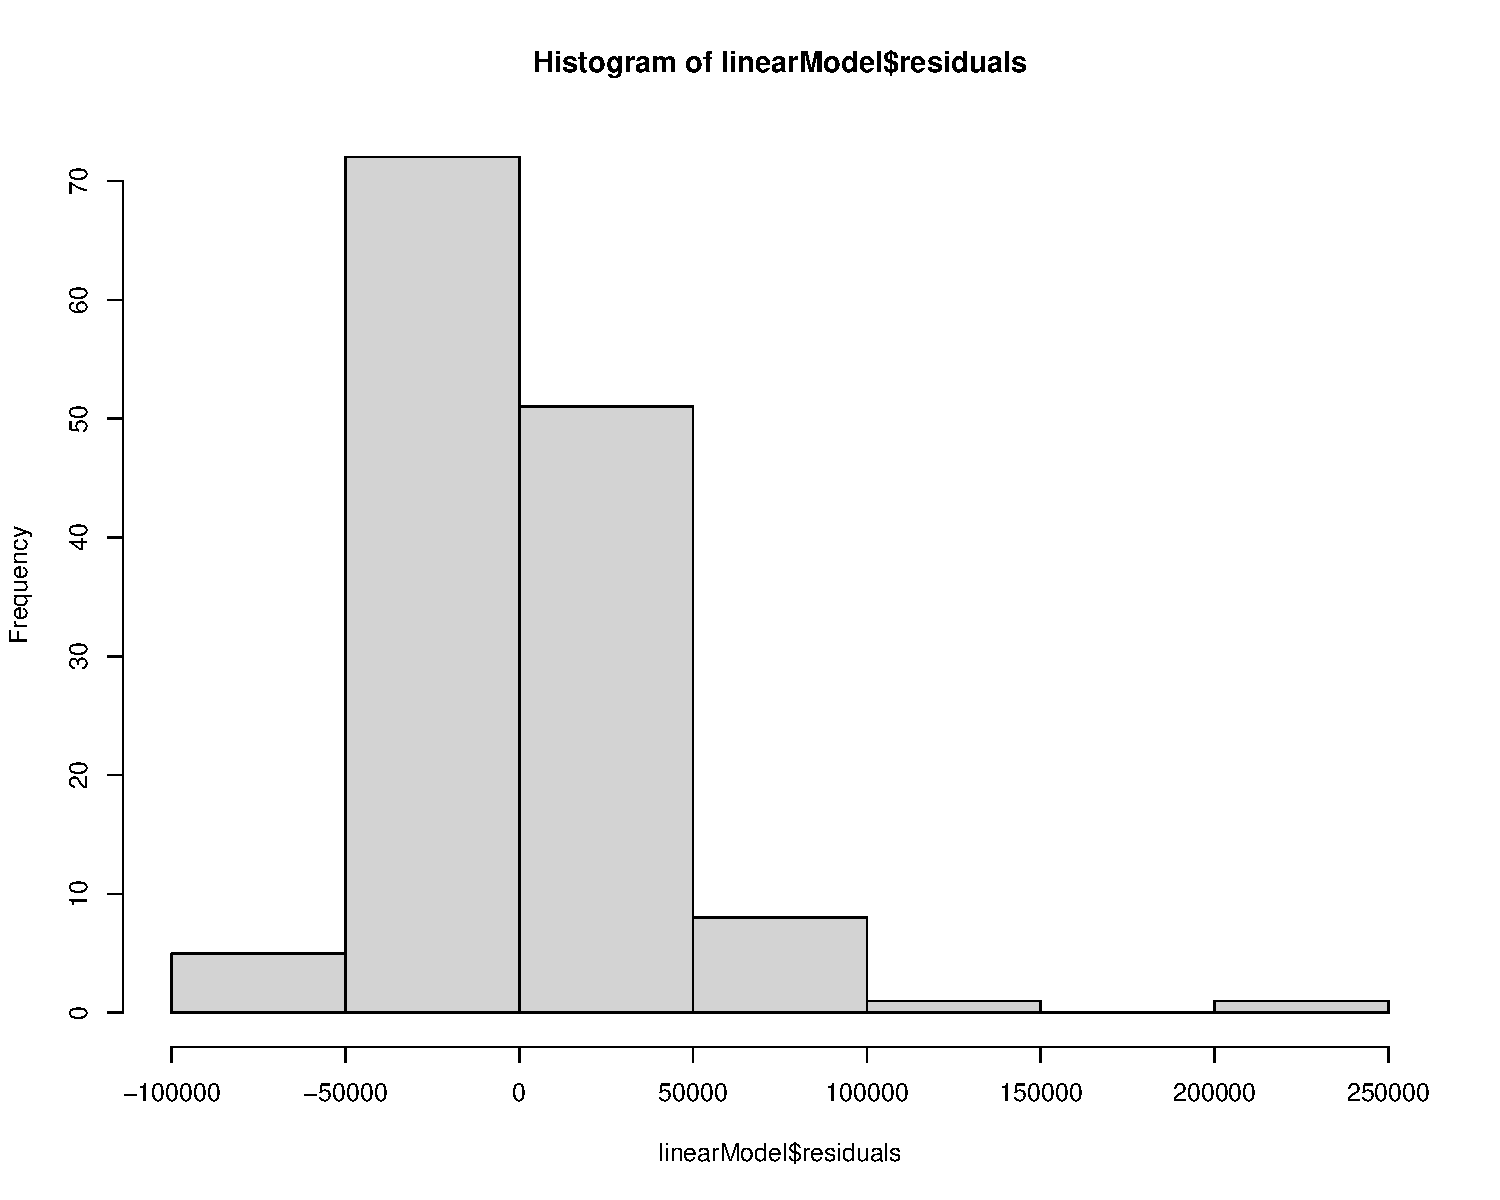
\includegraphics[width=0.6\textwidth]{./plots/caredaysResidualsHist.pdf}
  \caption{caption}
\end{figure}

Normalfordelingsplottet er ikke symmetrisk så det er ikke nødvendigvis
normalfordelt, og vi ser også her den ekstreme observation.

% Konklusion

\section{Opgave 3}

Vi opstiller en er en korrelationsmatrix. Denne viser at varibler som alder, køn
og forsikring ikke har en stor indvirkning.

% Konklusion
\begin{figure}[H]
  \centering
  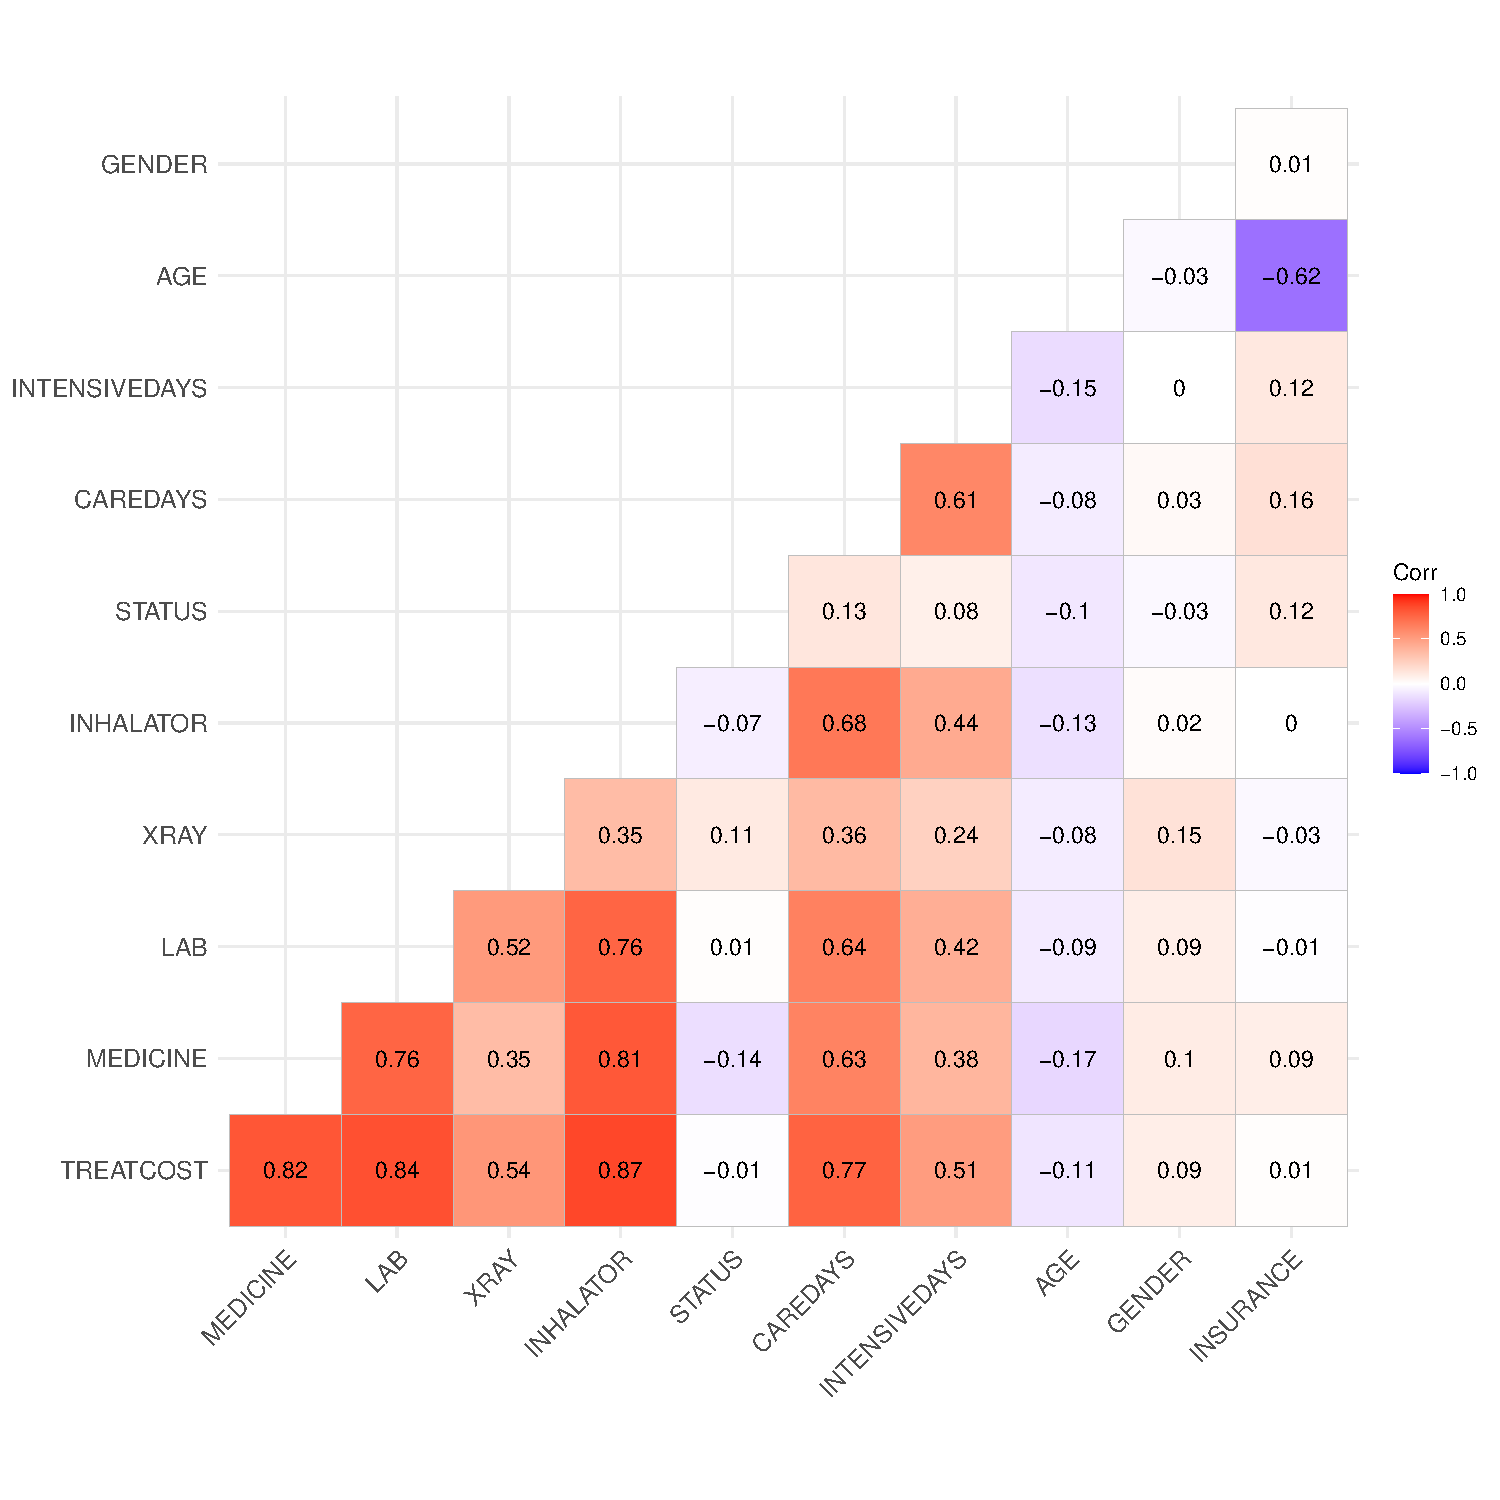
\includegraphics[width=0.6\textwidth]{./plots/corretlationMatrix.pdf}
  \caption{caption}
\end{figure}


Vi skal elimiere de varibler der ikke er ikke er vigtige for modellen, da den
mest komplekse model (den fulde model) ikke altid er den bedste. Til at
eliminere variabler og maksimere $ R^2_{adj} $ elimineres de variabler der ved
eliminering giver den højeste $ R^2_{adj} $. 

Efter at have elimineret status, age og gender ender vi med en model der ser
således ud: 
MEDICINE+LAB+XRAY+INHALATOR+CAREDAYS+INTENSIVEDAYS+INSURANCE. Dette giver en
forklaringsværdi på 0.888.

\section{Opgave 4}

Vi har en hypotese om at regionale forskellige kan have en indflydelse på brugen
af respirator, og de udgifter der følger med. Vi har en null hypotese $ H_0 $ og en
alternativ hypotese $ H_A $. Hvor null hypotesen udgør et konservativt synspunkt
og den alternative hypotese udgør noget nyere og mere interessant. 

\noindent$ H_0 $: Der er ingen regionale forskelle i brugen af respirator.\\
\noindent$ H_A $: Der er regionale forskelle i brugen af respirator.

Vi skal også bestemme et passende niveau for signifikans $ \alpha $. Hvis vælger
et lavere $\alpha$ fx $0.01$ er vi mindre tilbøjelige til at lave type 1 fejl
(hvor $ H_0 $ fejlagtigt afvises til fordel for  $ H_A $),
hvis vi vælger et højere $ \alpha $ fx 0.10 er vi mindre tilbøjelige til at lave type 2
fejl (hvor $ H_0 $ fejlagtigt ikke afvises). 
I forhold til vores hypotese betyder en type 1-fejl at der fejlagtigt
konstateres at der er regionale forskelle i brugen af respirator. 

\begin{figure}[H]
  \centering
  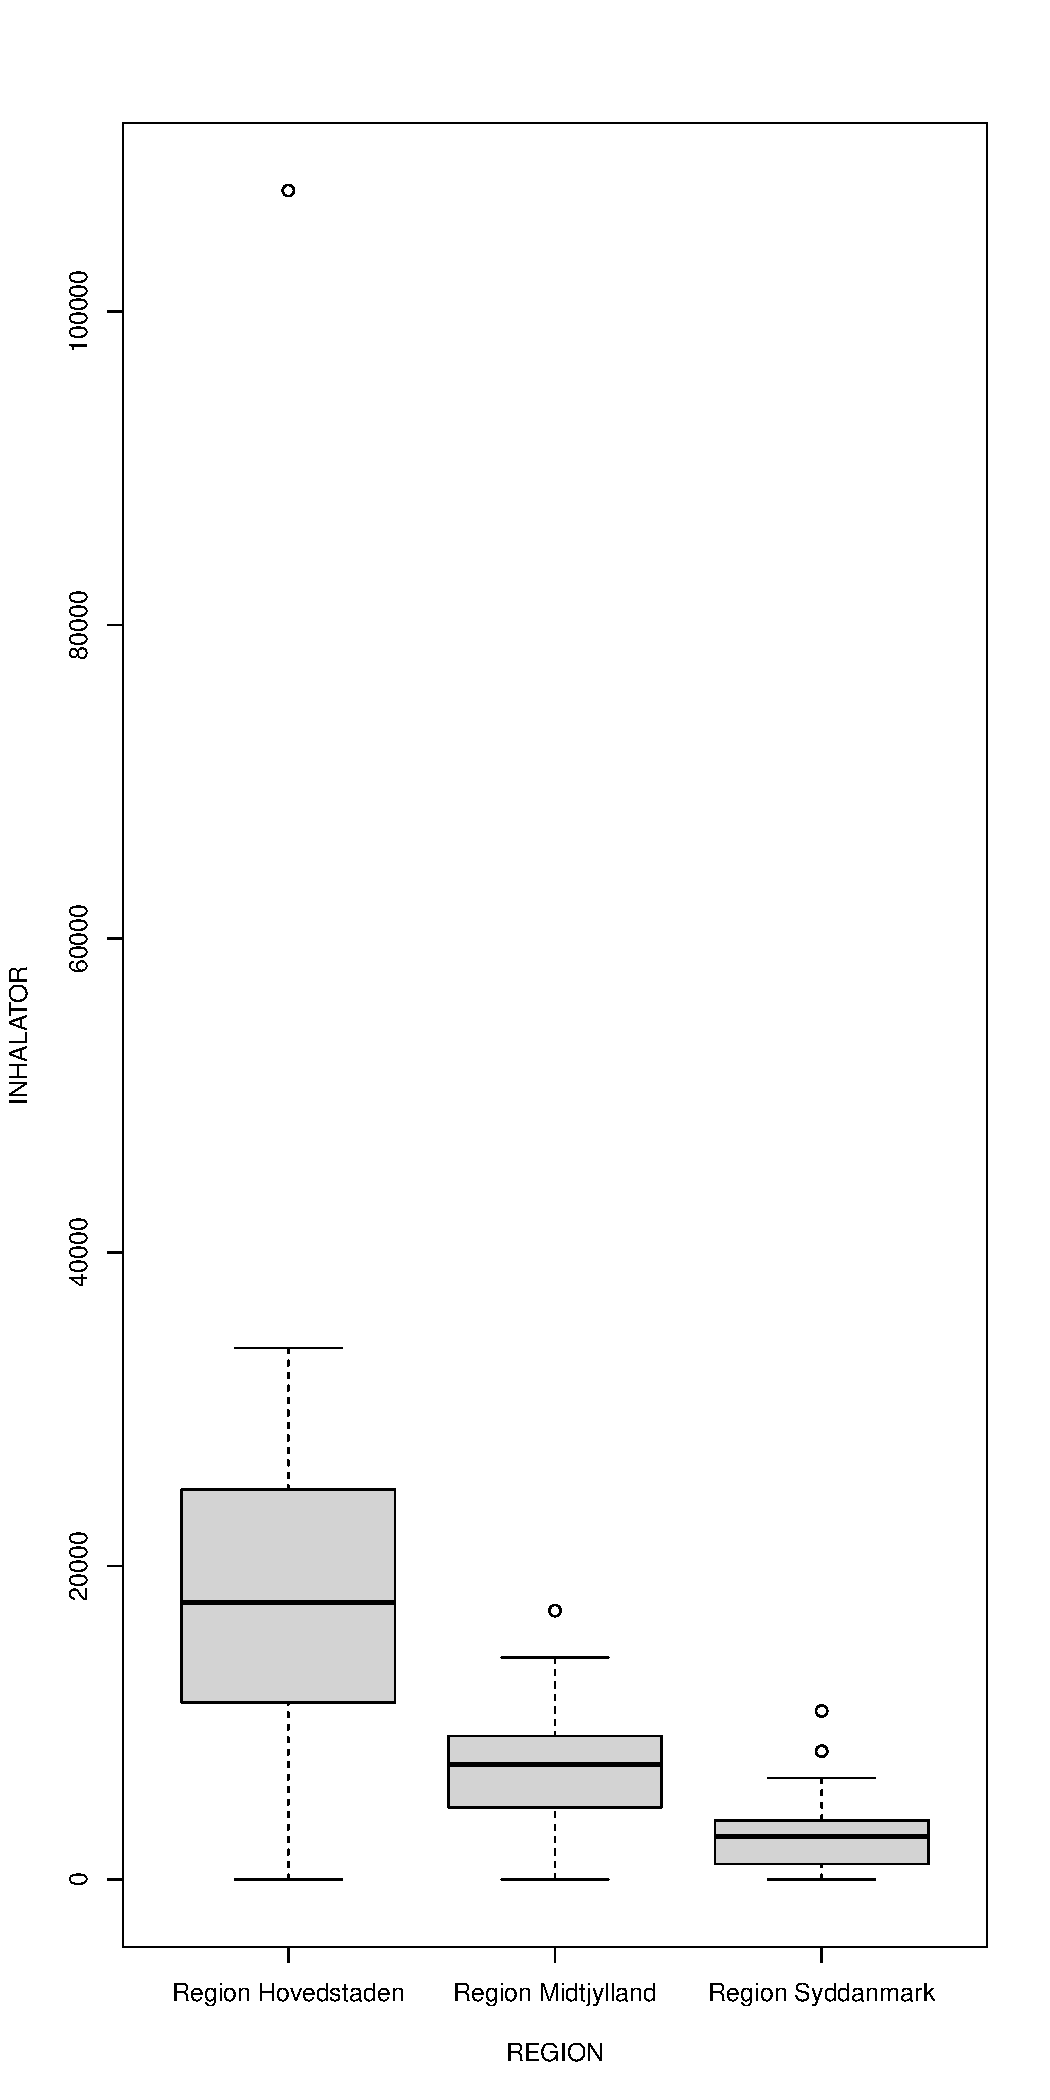
\includegraphics[width=0.8\textwidth]{./plots/anovaboxplot.pdf}
  \caption{caption}
\end{figure}

Resultatet af ANOVA viser signifikans.

% Konklusion

\section{Opgave 5}

Vi har en hypotese om at bestemte udgifter kan være relateret til køn, vi skal
undersøge om middeludgifterne til røntgenundersøgelser er højere for mandlige
end kvindelig patienter.


\section{R-kode}
\lstinputlisting[inputencoding=utf8/latin1, basicstyle=\\ttfamily]{aktivitet_2.R}
% Konklusion

\end{document}

